% Chapter 7

\chapter{Extracting the Weak Charge of the Proton}
\captionsetup{justification=justified,singlelinecheck=false}

\label{Ch:extracting_qwp}

\lhead{Chapter 7. \emph{Extracting \qwp}} 

The weak charge of the proton is determined by extrapolating the $Q^2$ dependence of the  parity-violating $ep$ scattering asymmetry to $Q^2=0$. This chapter serves to illustrate the process of taking the measured asymmetry and translating it into a value for the proton's weak charge. Extracting the weak charge requires a determination of the parity-violating asymmetry $A_{PV}$ from the measured asymmetry. Determining $A_{PV}$ requires many separate pieces of information, many of which are analysis topic in themselves, and which at the time of this writing are not yet mature. Furthermore, the final dataset may be expanded to include more data than were used in this analysis. To prevent unintentional bias toward the Standard Model prediction, the asymmetry dataset for the \Qs experiment is blinded, meaning that an undisclosed constant has been added to all asymmetry measurements. Until all pieces of information required to extract the weak charge from the measured asymmetry are finalized, the size of this blinding term will not be revealed. For these reasons what is presented in this chapter is intended for the purposes of illustration and will not represent the final result of \Q. This analysis will focus on the subset of Run 2 data for which a modulation correction exists.  

Determining the weak charge of the proton from the measured asymmetry can be divided into two analysis processes: the parity-violating asymmetry must be extracted from the measured asymmetry and some method must be employed for translating the parity-violating asymmetry measured at the kinematics of the \Qs experiment to $Q^2=0$. The parity-violating asymmetry evaluated at $Q^2=0$ is proportional to the weak charge of the proton (see Equation \ref{eq:reduced_asym}). The next two sections separately work through both of these processes to determine a final weak charge of the proton. For the measured asymmetry a straight average of the 16 PMT asymmetries will be used to eliminate bias introduced by unequal weighting. This average will be referred to as ``PMT Average''.

\section{\label{Sctn:qwpExtract}Extracting the Parity-Violating Asymmetry}
In Chapter \ref{Ch:instrumentation} the measured asymmetry was expressed as a sum of constituent parts, one of which was the parity-violating asymmetry of interest (see Equation \ref{eq:raw_asymmetry}). Using this equation to solve for the parity-violating asymmetry $A_{PV}$ gives
\begin{equation}
A_{PV}=\frac{R}{1-\sum_bf_b}\left[\frac{A_{meas}}{P}-\sum_bf_bA_b\right],
\label{eq:pv_asymmetry}
\end{equation} 
where the asymmetry $A_{meas}$ is the raw asymmetry corrected for helicity-correlated false asymmetries
\begin{equation}
A_{meas}=A_{raw}-A_{beam}-A_{bb}-A_T-A_{\epsilon}.
\label{eq:a_meas}
\end{equation} 

With a total of three backgrounds, there are 13 values that must be determined before the parity-violating asymmetry can be evaluated. Each of these is dealt with below.
\subsection{Bias Corrections}
$R$ is a multiplicative factor to account for changes from the measured to the reported $Q^2$ of the experiment and is the product of several factors which bias the asymmetry: $R=R_{RC}R_{Det}R_{Bin}R_{Q^2}$.

The experimental asymmetry will be reported at a given effective angle, beam energy and $Q^2$, whereas the detector accepted a range of angles and energies. Multiple scattering and {\it bremsstrahlung} processes, including higher order vacuum loops, alter the angle, energy and polarization of the electron both before and after scattering. The aim is to report the ``tree level'' parity-violating asymmetry rather than the measured asymmetry which includes radiative effects. $R_{RC}=\frac{A_{tree}}{A_{RC}}$ comes from the GEANT3 simulation for \Qs and is the ratio of the simulated asymmetry without radiative effects to the asymmetry with radiative effects. For Run 2, this factor is estimated to be $R_{RC}=1.0101\pm 0.0007$.

A detector light-weighting correction is required due to the non-uniformity of the distribution of $Q^2$ across the detector bars, coupled with position/angle dependent production and collection of \v{C}erenkov light. GEANT4 simulations comparing light-weighted $Q^2$ distributions to those without light weighting gave a correction factor to the measured asymmetry of $R_{Det}=0.9921\pm 0.0044$ . 

$R_{Bin}$ is a factor which corrects the measured asymmetry which is averaged over the accepted $Q^2$ distribution, $\left<A(Q^2)\right>$, to the reported asymmetry at a single $Q^2$ value, $A(\left< Q^2\right>)$. This factor was determined by simulation to be $R_{Bin}=0.98\pm 0.005$. Although this is a model-dependent correction, its sensitivity to the parametrization used to extract the $Q^2$-dependence of the asymmetry is negligible.

With an additional systematic error of 0.016 to account for the uncertainty in determining the central $Q^2$ upon which all the other factors depend, the total correction factor $R$ becomes
\[
 R=R_{RC}R_{Det}R_{Bin}R_{Q^2}=0.982\pm 0.019.
\]

\subsection{Background Corrections}
There are three sources considered as background contributions to the measured asymmetry in \Q. For each of these, the best estimates are given at the time of writing for both the size of the background $A_b$ and the fraction to which it contributes to the observed detector yield $f_b$.  
\begin{itemize}
\item{The largest background comes from the aluminum entrance and exit windows on the target. A thick 4\% (0.04 radiation lengths) aluminum target made from the same material as the target windows and located near the position of the downstream aluminum window was used to measure the size of the asymmetry. The measured asymmetry was scaled individually for the upstream and downstream windows to account for differences in asymmetry between the thick target and the windows as follows:
\[
A_{u,d}=A_{4\%}\frac{A_{u,d}^{sim}}{A_{4\%}^{sim}},
\]
where $A_{u(d)}$ are the asymmetries for the upstream (downstream) windows and $A_{4\%}$ is the asymmetry measured on the thick aluminum target. The simulation corrects for changes due to $z$-location, energy loss in the hydrogen target, as well as radiative effects associated with a thicker target material. Included in the simulation are generators for elastics, quasi-elastics, inelastics, inelastic single particle states and giant dipole resonances. The total asymmetry is calculated as \
\[
A_{windows}=\frac{R_uA_u+R_dA_d}{R_u+R_d},
\]
where $R_{u(d)}$ is the detector rate coming from the upstream (downstream) windows. The total polarization-corrected asymmetry is $A_1=1506\pm 72$~ppb. 

The dilution fraction from the aluminum windows is measured to first order as $f_{win}=\frac{Y_{empty}}{Y_{full}}$, where $Y_{empty}$ is the current-normalized detector yield with an evacuated target and $Y_{full}$ the current-normalized detector yield with the target full of liquid hydrogen. This ratio needs to be corrected for energy losses associated with the presence of liquid hydrogen. Without the hydrogen in the target the image of the upstream aluminum window mostly falls off the bar. A light-weighting correction needs to be applied to translate the measured rates to light yields in the detector bars. The corrected dilution fraction for the aluminum windows is $f_1=0.02590\pm 0.00011$.}
\item{A second background is a soft neutral background arising from secondary electron scattering from collimator edges, the shielding wall and the \qtor spectrometer along the scattered electron transport channel. For this reason it is often referred to as the ``QTOR transport channel'' background. The dilution fraction for this background was measured using the Region 3 trigger scintillator detectors. The two scintillator detectors, used during tracking mode, were situated in opposite octants and could be rotated to cover the acceptance of any two opposite detector bars (see Figure \ref{fig:vdcs}). Since the scintillators were insensitive to neutral particles, they were used as a vetoes for the main detector, accepting only events that fired the main detector but not the trigger scintillator. The dilution fraction was measured to be $f_2=0.0013\pm 0.0014$. The asymmetry associated with this background is taken from simulation and the best estimate as of this writing is $A_2=-283\pm 57$~ppb }
\item{A third background comes from inelastic scattering events associated with $N\rightarrow \Delta(1232)$ production. Figure \ref{fig:sim_current_scan} illustrates the presence of the inelastic distribution tail under the elastic peak at a spectrometer current of 8921~A where production data was taken. The dilution fraction of the inelastic distribution was determined using simulation to be $f_3=0.0002\pm 0.0002$. The asymmetry associated with this inelastic process was measured at the inelastic peak by reducing the spectrometer current to 6700~A where the inelastic peak was focused on the detector bars. This asymmetry was corrected for an elastic radiative tail, the aluminum window, and neutral backgrounds. The corrected inelastic asymmetry under the production elastic peak at 8921~A was determined to be $A_3=-3020\pm970$~ppb.}
\end{itemize}
\begin{figure}[ht]
\begin{center}
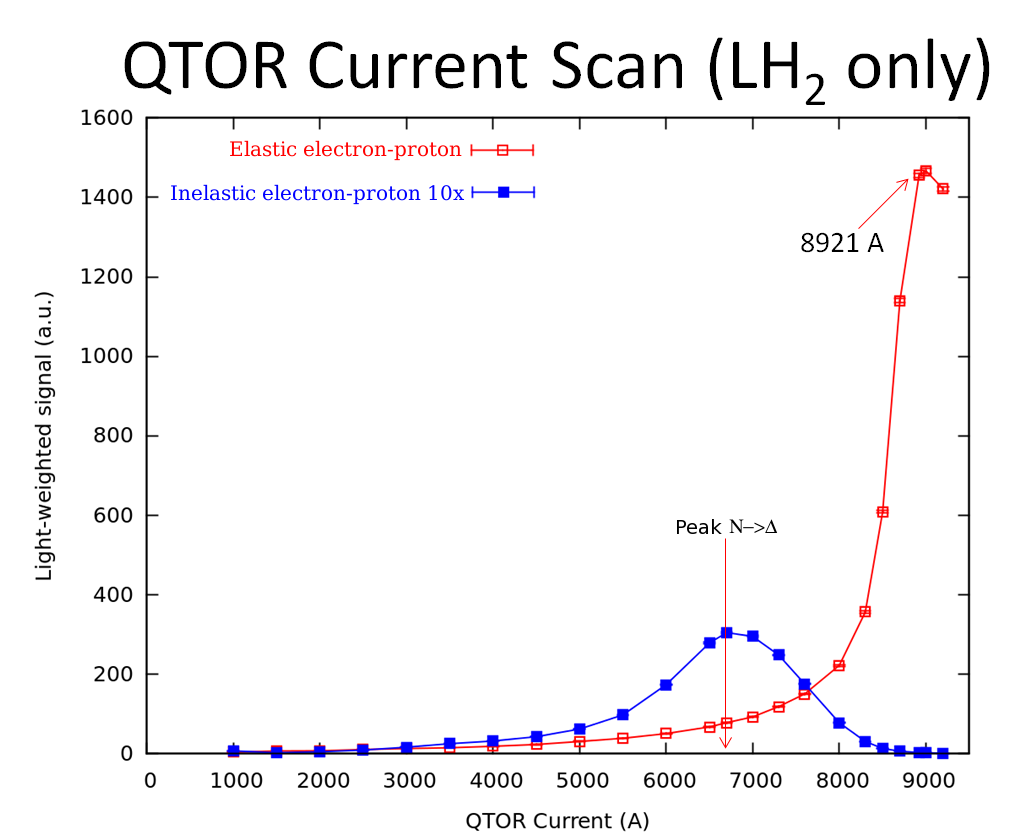
\includegraphics[width=4in]{./Pictures/qtor_current_scan.png}
\caption{\label{fig:sim_current_scan}Simulation of liquid hydrogen (LH2) elastic and inelastic scattering events versus \qtor spectrometer current clearly showing the peak $N\rightarrow\Delta$ production at 6700~A. The tail of the inelastic distribution under the elastic peak creates the fourth background asymmetry $A_3$.}
\end{center}
\end{figure}
Therefore the total background asymmetry correction is 
\[
A_{Bkgd}=\sum_{b=1}^3f_bA_b=38.0\pm2.0~\text{ppb}
\] 
and the fraction of the measured yield coming from elastic electron-proton scattering is 
\[
f_{ep}=1-\sum_{b=1}^3f_b=0.9726\pm 0.0014.
\]
\subsection{Measured Asymmetry}
The measured asymmetry $A_{meas}$ given by Equation \ref{eq:a_meas} is composed of the raw asymmetry with helicity-correlated false asymmetries subtracted off. Of these false asymmetries, only two have signficant corrections to apply:  $A_{beam}$, a false asymmetry associated with with helicity-correlated beam motion, and $A_{bb}$, a false asymmetry associated with a neutral background seen in the main detector.

The error-weighted raw asymmetry $A_{raw}$ for the main detector PMT average over the Run 2 data set was $-159.4\pm 8.2$(stat)~ppb. Runlet-level (4-5 minute) averages of the main detector asymmetry distribution were first calculated. The error for each runlet-level asymmetry was calculated as the RMS width of the distribution divided by the square root of the number of quartets in the runlet. The total asymmetry was then calculated as the error-weighted average of runlet-level asymmetries \footnote{The runlet-level error weights were determined as the inverse variance of the modulation-corrected quartet MDallbars asymmetry distributions divided by the number of quartets in the runlet ($\frac{1}{\sigma^2_{quartet}/N_{runlet}}$)}. This total asymmetry measurement includes a total of 760542988 quartets\footnote{Recall that 1 quartet is approximately 4~ms of data.} and has a PMT-average quartet asymmetry RMS width of 225.4~ppm.  

Detector non-linearity, bounded by bench tests of the PMT + readout electronics, was estimated to be less than 1\%. An uncertainty of 2~ppb is assigned to account for this potential source of systematic error.   

\Qs operated as a ``blinded'' experiment, meaning that the reported asymmetries were offset from their true value by an additive constant. As previously mentioned, this blinding was done as a barrier to prevent unintentional biasing of the data toward the Standard Model expectation during the analysis process. The blinding term, selected from a uniform distribution over the range $\pm 60$~ppb, was added to each quartet-level asymmetry. Blinding was implemented in the software analyzer such that the raw data remained untouched but all processed files had the blinding term added to main detector calculated asymmetries. This blinding term remains a secret at the time of writing and will only be unveiled after all the data analysis is complete. As a result, the asymmetry quoted in this analysis is blinded.

The correction $A_{beam}$ is associated with helicity-correlated beam parameters position, angle, and energy. The details of this correction were given in Chapter \ref{Ch:BMod_correction}. For Run 2 this correction is $A_{beam}=-2.1\pm 0.8$~ppb.

$A_{bb}$ is a false asymmetry associated with helicity-correlated scattering in the beamline downstream of the target. This background was measured to be independent of spectrometer current implying that it is neutral particles and is believed to be primarily created in the tungsten collimator just downstream of the target. This background asymmetry was studied by blocking octants 1 and 5 of the primary collimator with 5~cm of tungsten. Asymmetries measured in main detector bars 1 and 5 during blocked octant running were seen to be highly correlated with the three background detectors (PMTonly, PMTltg and MD9) as well as the upstream luminosity monitors, giving evidence that they were all observing the same background. Since the luminosity monitors provide the most statistically accurate measure of the background asymmetry, they were chosen as the natural candidate for monitoring the background asymmetry during production running. The correlation between slug-level ($\sim$8~hr blocks of data) averages of the main detector and the upstream luminosity monitors over Run 2 provides a scale factor $\alpha$ for correcting the main detector asymmetry as follows:
\[
A_{bb}=\alpha A_{bb}^{uslumi},
\]
  
where $A_{bb}^{uslumi}$ is the beamline background asymmetry seen in the upstream luminosity monitor. This scale factor $\alpha=3.9\pm 1.5$~ppb/ppm, was determined from this correlation over Run 2. The asymmetry of the upstream luminosity monitors averaged over Run 2 is  $A_{bb}^{uslumi}=0.99$~ppm (sign-corrected for slow helicity reversals), giving a total correction $A_{bb}=3.9\pm2.2$~ppb.

$A_T$ is the false asymmetry from residual transverse polarization on the electron beam. The parity-conserving scattering asymmetry associated with a fully transverse-polarized beam was measured to be $-4.8\pm 0.6$~ppm \cite{Waidyawansa}. Although the \Qs experiment nominally ran with longitudinally polarized beam, evidence of a residual transverse polarization remained. Transverse electron polarization manifests itself as an azimuthal dependence of the scattering asymmetry in the main detector. Figure \ref{fig:transverse_fit} shows the azimuthal dependence of the average asymmetry over Run 2 with a sinusoidal fit to find the residual of the transverse polarization projected into its horizontal and vertical components. For Run 2, the residual vertical transverse polarization was $P_V=-0.0095$ and the residual horizontal transverse polarization was $P_H=0.0023$, which corresponds to a rotation of the ``polarization vector'' by $0.5^{\circ}$ vertically and $0.1^{\circ}$ horizontally from perfect longitudinal polarization.
\begin{figure}[ht]
\begin{center}
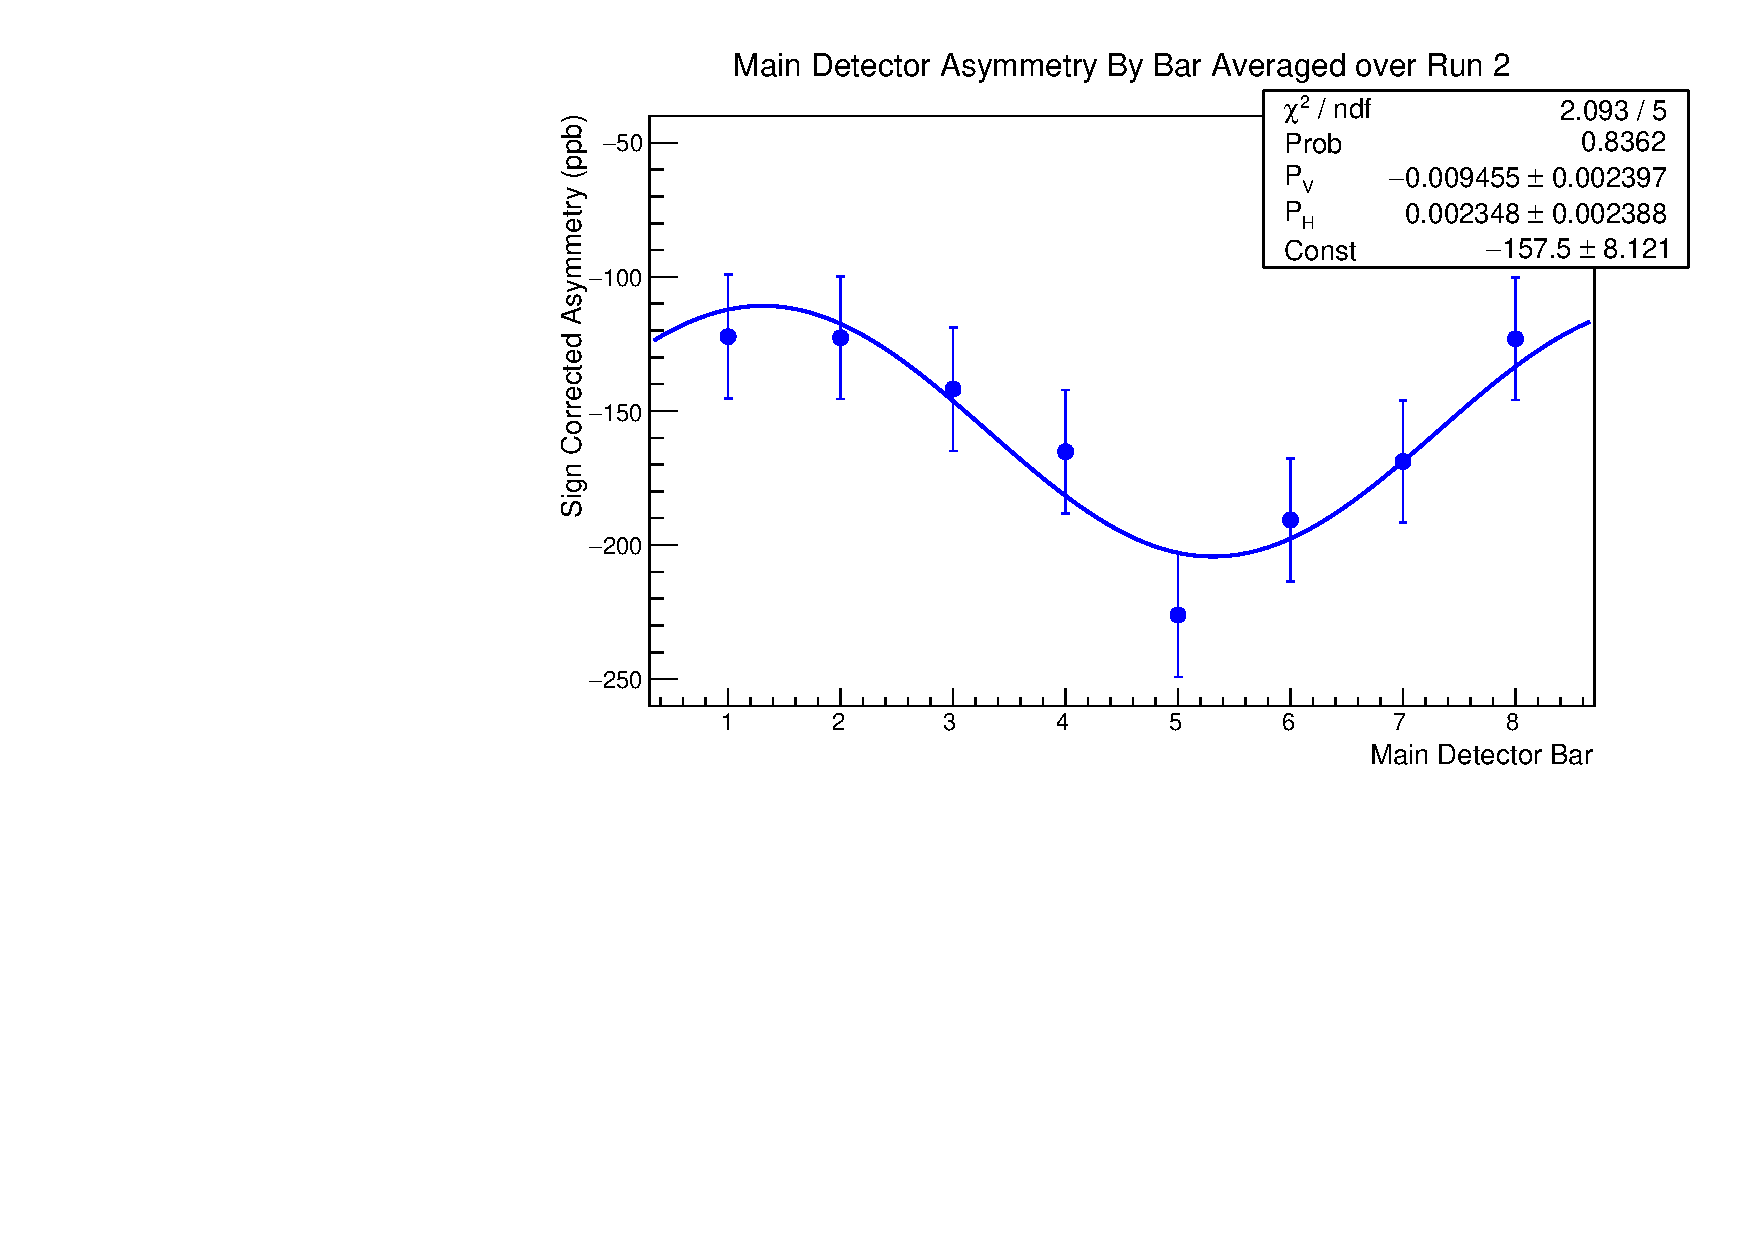
\includegraphics[width=4in]{./Pictures/transverse_fit.pdf}
\caption{\label{fig:transverse_fit}Modulation-corrected (and sign-corrected for slow helicity reversals) PMT average  asymmetry by bar showing manifest azimuthal dependence. The values shown are averages over Run 2 and the following function is fit to the data: $-4800\times\left[P_V\cos{\left(\frac{Bar\#-1}{4\pi}\right)-P_H\sin{\left(\frac{Bar\#-1}{4\pi}\right)}}\right]+Const$. $P_{V(H)}$ is the vertical (horizontal) transverse polarization.}
\end{center}
\end{figure}

To first order the transverse asymmetry cancels around the azimuth but broken symmetries in the main detector slightly degrade this cancellation, creating a small leakage term. Details on the method of extracting the leakage are provided in \cite{Waidyawansa}. The azimuthal dependence of the detectors was fit during separate running periods with maximal horizontal and vertical transverse polarizations. The fit similar to that shown in Figure \ref{fig:transverse_fit} was performed. The constant term of the fit measures the lack of cancellation. The constant leakage terms for the horizontal and vertical transverse polarizations were measured to be $C_H=11\pm 61$~ppb and $C_V=12\pm 55$~ppb respectively. Both are consistent with zero, but the upper bound is given by the large uncertainty. The transverse leakage is given as  
\[
A_T=\left|C_V\times P_V\right|+\left|C_H\times P_H\right|=0.14\pm0.55~\text{ppb.}
\]
Because the correction is negligible relative to the its error, it will be assumed to be zero and only the uncertainty of $\pm0.6$~ppb will be applied. 

 The false asymmetry associated with electronics pickup correlated with the helicity reversal was measured to be consistent with zero over Run 2 with high precision using a null channel. Figure \ref{fig:isourc_asym} shows the measured distribution of a current source (battery) plugged into one of the \Qs data acquisition channels. The signal in this channel was adjusted to approximately the same level as the detector channels so that the effect of helicity pickup for the battery channel would be similar to that of the detectors. The mean asymmetry of -0.02$\pm$0.09~ppb is consistent with zero and completely negligible.

Putting all this together gives 
\[
A_{meas}=A_{raw}-A_{beam}-A_{bb}=-161.2\pm 8.2\text{(stat)}\pm3.1\text{(sys)~ppb},
\]
where errors are included from statistics, the modulation correction, the beamline background correction, transverse leakage and detector non-linearity.
\begin{figure}[ht]
\begin{center}
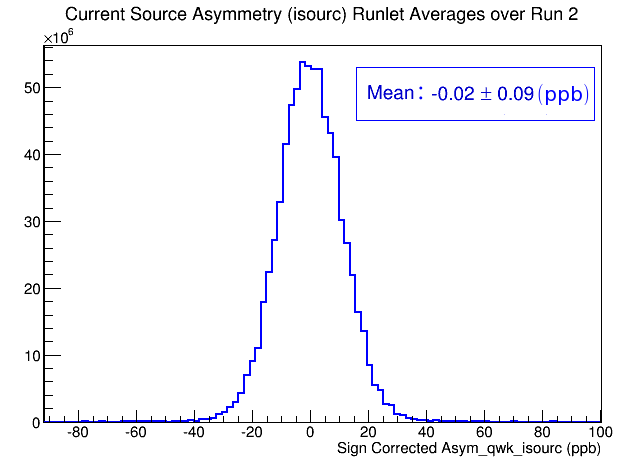
\includegraphics[width=3.5in]{./Pictures/isourc_asym.png}
\caption{\label{fig:isourc_asym}Distribution of asymmetry measurements of a battery fed channel in the \Qs data acquisition. Data has been corrected to reverse sign with slow helicity reversals so that it can be directly compared with the parity-violating physics asymmetry. The distribution is formed of runlet level averages (4-5 minute averages) weighted by the number of quartets in the runlet. The error on the mean is calculated by the average quartet RMS width divided by the square root of the total number of quartets (7.57e8 quartets)\protect\footnotemark.}
\end{center}
\end{figure}
\footnotetext{The cut applied to the dataset including isourc was different from that applied to the main detector dataset in the analysis of the past chapter. This resulted in 0.5\% fewer quartets in for the isourc asymmetry. This difference does not alter the conclusions.} 

\subsection{Polarization}
The electron polarization was determined using a combination of the Compton electron detector and M\o ller polarimeters. The electron detector delivered continuous polarizations at nominal running conditions and its values were chosen to give the time-dependent polarization. A small systematic difference of 0.7\% was observed between Compton and M\o ller values averaged over Run 2. Given the systematic error of 0.83\% reported for the M\o ller and 0.58\% for the Compton (see Chapter \ref{Ch:instrumentation}), this difference is not alarming. The reported polarization was weighted to include both. The total relative error for the polarization over Run 2 including both systematic and statistical errors is 0.62\%. The yellow bands in Figure \ref{fig:run2_epol} show the scaled polarization values and errors over Run 2. The polarization for the data set included in this analysis, averaged with the same weights as are applied to the main detector asymmetry, is $P=0.889\pm0.006$.
\begin{figure}[!h]
\begin{center}
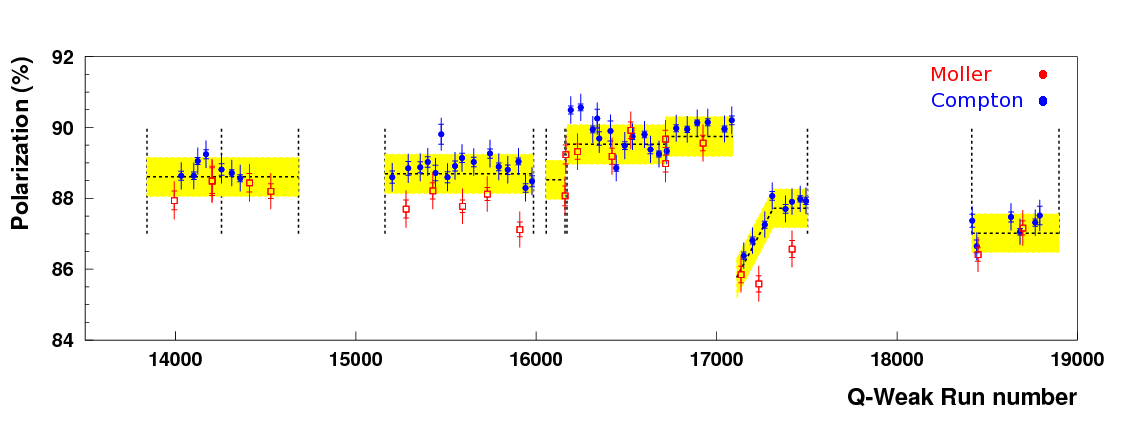
\includegraphics[width=5.9in]{./Pictures/qweak_run2_polarization_v2.png}
\caption{\label{fig:run2_epol}The electron beam polarization values for the Compton electron detector and the M\o ller polarimeter over Run 2. The yellow bands represent the central value and full error (systematic and statistical) for the given period.}
\end{center}
\end{figure}

\subsection{The Parity-Violating Asymmetry}
Re-expressing Equation \ref{eq:pv_asymmetry} in simpler terms, the parity-violating asymmetry is then given as

\begin{equation}
A_{PV}=\frac{R}{f_{ep}}\left(\frac{A_{meas}}{P}-A_{Bkgd}\right)= -221.5\pm 9.3\text{(stat)}\pm 6.1\text{(syst)~ppb}.
\label{eq:apv_exp}
\end{equation}
The total error added in quadrature is 11.1~ppb. Values and errors for the individual terms in the expression are summarized in Table \ref{tab:asym_err}.



\begin{table}[h]
\begin{center}
\caption{\label{tab:asym_err}Summary of values and errors for various terms in the calculation of the parity-violating asymmetry $A_{PV}$. }
\begin{tabular}{|l|c|p{5cm}|}\hline
Term&Value&Comment\\\hline\hline
R&0.982$\pm$0.019&$R=R_{RC}R_{Det}R_{Bin}R_{Q^2}$\\\hline
P&0.889$\pm$0.006&Electron beam polarization\\\hline
$A_{meas}$&$-161.2\pm$8.2(stat)$\pm$3.1(sys)~ppb&Error includes statistics, non-linearity, transverse leakage, and modulation correction\\\hline
$f_{ep}$&0.9726$\pm$0.0014&$f_{ep}=1-\sum_{b=1}^3f_b$\\\hline
$A_{Bkgd}$&38.0$\pm$2.0~ppb&$A_{Bkgd}=\sum_{b=1}^3f_bA_b$\\\hline
\end{tabular}
\end{center}
\end{table}

As detailed in Chapter 3, each of the eight main detector bars are read out by two PMT's, one at each end. The PMTavg Asymmetry (straight average of the 16 PMT asymmetries) gives the physics asymmetry for \Q. An interesting/troubling phenomenon has been found in the \Qs production data. A well-determined discrepancy exists between the asymmetries measured by the two PMT's on each detector bar, although both are collecting light from the same quartz bar, albeit from opposite ends. Figure \ref{fig:pmt_dd} shows this discrepancy between the asymmetry measured on the opposite ends of each bar. This difference in asymmetry, measured to be uniform in all octants of the main detector and stable over time, has been termed the ``PMT double difference''. This effect is believed to originate from transverse polarization of the scattered electrons arising from g-2 precession as the electrons travel through the \qtor spectrometer which rotates the electron spin $\sim 35^{\circ}$ relative to its trajectory. These electrons then scatter and shower in the lead pre-radiators on the front of each main detector bar. Non-uniformity of light collection as a function of angle and position along the detector bar, coupled with a small polarization-dependent shift in the event distribution, is believed to cause this discrepancy. Two models currently being simulated show promise of contributing to this effect. GEANT4 simulations of spin-dependent Mott scattering of transversely polarized electrons which have radiated to low energies in the pre-radiators, appear to show a small polarization-dependent distribution shift. Another model being simulated is the higher energy parity-conserving transverse scattering asymmetry from the analyzing power in lead, with an effect similar to that measured by \Qs for scattering from the proton \cite{Waidyawansa}. 

Analysis of this effect is ongoing. In either of these models, the double difference effect will cancel in the average of all PMT's to first order. Broken symmetries in the main detector ensure this cancellation will not be perfect. However, light sensitivity distributions measured using the tracking system will allow a correction for this leakage of the double difference into the PMT average asymmetry. Conservatively estimating the leakage due to broken detector symmetry at $\pm$10\% and a correction factor calculated from tracking data known to the $\pm$10\% level would give a systematic uncertainty of 1\% to the correction of the 300~ppb double-difference. Although at this point it is premature to assign an uncertainty for this effect and it will not be considered in this analysis, the reader should keep in mind that this effect will contribute to the final uncertainty of the unblinded result.

\begin{figure}
\centering
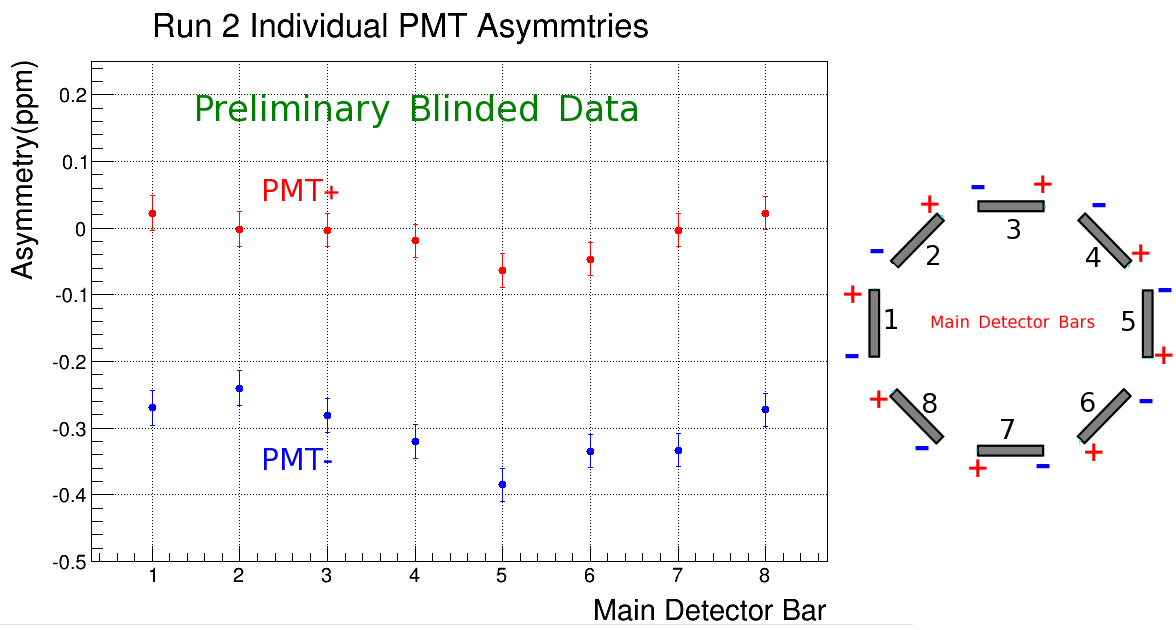
\includegraphics[width=5.8in]{./Pictures/PMT_DD.png}
\caption{\label{fig:pmt_dd}Main detector asymmetries averaged over Run 2 showing the systematic difference between positive and negative PMT's. This ``PMT double-difference'' effect is uniform in all octants. The sinusoidal variation around the azimuth arises from residual transverse polarization on the electron beam and is a distinct from the double-difference believed to arise from transverse polarization of the scattered electrons produced by g-2 precession in the spectrometer. }
\end{figure}

\section{\label{Sctn:qwpExtract}From Parity-Violating Asymmetry to Weak Charge}
To obtain the weak charge of the proton, \qwp, from the measured parity-violating asymmetry, recall the following equation introduced in Chapter 2.
\begin{equation}
A_{PV}/A_0=\left[\frac{{\epsilon}G^{\gamma,p}_EG^{Z,p}_E+{\tau}G^{\gamma,p}_MG^{Z,p}_M-\left(1-4\sin^2{\theta}_W\right){\epsilon}^{\prime}G^{\gamma,p}_MG^{Z,p}_A}{{\epsilon}(G^{\gamma,p}_E)^2+{\tau}(G^{\gamma,p}_M)^2} \right],
\label{eq:qw_asymmetry2}
\end{equation} 
with $A_0=\frac{-G_FQ^2}{4\pi \alpha\sqrt{2}}$.
The electromagnetic Sachs form factors of the proton, $G^{\gamma,p}_E$ and $G^{\gamma,p}_M$, are well-determined from parity-conserving electron scattering. Values for the weak neutral current (WNC) vector form factors can be derived from measured electromagnetic form factors of the proton and neutron under the assumption of charge symmetry which asserts the invariance under the following interchanges: $p\leftrightarrow n$, $u\leftrightarrow d$ and $s\leftrightarrow s$. Here $p~(n)$ are proton (neutron), $u~(d)$ are up (down) quarks and $s$ is the strange quark\footnote{Contributions from heavier quarks are neglected. In fact, for the purposes of this analysis it is appropriate to drop the strange contribution as well}. Thus charge symmetry implies that the form factors of the up (down) quark for the proton are identical to the form factors for the down (up) quark of the neutron and that strangeness contributes equally to both. The effect of charge symmetry breaking is expected to alter the electromagnetic form factors less $1\%$ at the kinematics of \Q\cite{Miller2014}. Expressing the form factor of the proton and neutron in terms of the quark distributions $G_{E,M}^u$, $G_{E,M}^d$ and $G_{E,M}^s$ weighted by their electric charges gives 
\begin{equation}
G_{E,M}^{\gamma p}=\frac{2}{3}G_{E,M}^{u}-\frac{1}{3}(G_{E,M}^{d}+G_{E,M}^{s}).
\label{eq:gemp}
\end{equation}
Using the same distributions under the assumption of charge symmetry yield the following for the neutron:
\begin{equation}
G_{E,M}^{\gamma n}=\frac{2}{3}G_{E,M}^{d}-\frac{1}{3}(G_{E,M}^{u}+G_{E,M}^{s})
\label{eq:gemn}
\end{equation}
Rearranging these equations allows the quark form factors to be expressed in terms of the measured proton and neutron form factors plus an addition from strangenes:
\begin{align}
G_{E,M}^u=2G_{E,M}^{\gamma p}+G_{E,M}^{\gamma n}+G_{E,M}^{s}\\
G_{E,M}^d=G_{E,M}^{\gamma p}+2G_{E,M}^{\gamma n}+G_{E,M}^{s}
\label{eq:qFFs}
\end{align}
The WNC vector form factor $G_{E,M}^{Z p}$ can also be expressed in terms of the quark form factors weighted with the appropriate weak charges
\begin{equation}
\begin{array}{lcc}
G_{E,M}^{Zp}&=&\left(1-\frac{8}{3}\sin^2\theta_W\right)G_{E,M}^u+\left(-1+\frac{4}{3}\sin^2\theta_W\right)(G_{E,M}^d-G_{E,M}^s)\\
~&=&\left(1-4\sin^2\theta_W\right)G_{E,M}^p+(-1)(G_{E,M}^n-G_{E,M}^s)\\
~&=&Q_W^pG_{E,M}^p+Q_W^nG_{E,M}^n-G_{E,M}^s\end{array},
\label{eq:gemzp}
\end{equation}
where the proton and neutron measured form factors have been substituted using Equations \ref{eq:qFFs}. In the final line the form factor weights have been labeled to clearly show that they are the weak charges of the proton and neutron. At $Q^2=0$, the WNC electric form factor $G_{E}^{Zp}$ gives the weak charge of the proton. 

In the following analysis, strange quark content will be assumed to be zero. Strange content of the proton form factors measured by the HAPPEX-III experiment was found to be consistent with zero\cite{HAPPEX3}. Recently-published lattice QCD results provide even tighter constraints on form factor strange quark content, with evidence of non-zero strangeness but at levels that are negligible for this analysis\cite{Green2015}. Estimates based on figures in \cite{Green2015} suggest the following contributions to the form factors:
\begin{align}
G_E^s\left(Q^2=0.025(Gev/c)^2\right)=0.0006\pm0.0002\\
G_M^s\left(Q^2=0.025(Gev/c)^2\right)=0.017\pm0.004.\\
\end{align}
These enter the nucleon form factors (Equations \ref{eq:gemp} and \ref{eq:gemn}) weighted by the strange quark charge (-1/3). With estimates of the proton electric and magnetic form factors at the \Qs kinematics of the following size,
\begin{align*}
G_E^p\left(Q^2=0.025(Gev/c)^2\right)\approx 0.9\\
G_M^p\left(Q^2=0.025(Gev/c)^2\right)\approx 2.6,
\end{align*}
strange quark contributions to the form factors are expected to be less than 0.3\%. A further suppression by a factor of 3 comes from the fact that the form factors only contribute to the hadronic correction terms, which are about 33\% of $A_{PV}$ at the kinematics of \Q.

For the analysis ahead, the formalism outlined in \cite{Lui2007} is followed. The parity-violating asymmetry is re-expressed in terms of proton and neutron form factors giving
\begin{equation}
\begin{array}{lcl}
A_{PV}/A_0&=&(1-4\sin^2\theta_W)(1+R_V^p)\\~&~&-\left[\left(\epsilon G_E^{\gamma p}G_E^{\gamma n}+\tau G_M^{\gamma p}G_M^{\gamma n}\right)(1+R_V^n)+\epsilon^{\prime}(1-4\sin^2\theta_W)G_M^pG_A^e\right]/\sigma_{red},\end{array}
\label{eq:apv_pnFFs}
\end{equation} 
where 
\[
\tau=Q^2/(4M_p^2),~~~~\epsilon=(1+2(1+\tau)\tan^2\theta_e)^{-1},~~~~\sigma_{red}=\epsilon (G_E^{\gamma p})^2+\tau (G_M^{\gamma p})^2,
\]
and $\theta_e$ is the electron scattering angle. The factors $R_{V}^p$ and $R_V^n$ are radiative corrections that are both $Q^2$ and process-dependent and are required to correct for higher order lepton-quark scattering diagrams. The values for $R_V^{p,n}$ are given in Table \ref{tab:Apv_parameters}. 

Fits to world electron scattering data have yielded precise functional parametrizations of the form factors \cite{Galster}\cite{Walcher}\cite{Kelly}\cite{ArringtonSick}\cite{Venkat}. Of these schemes, the form factor parametrization by Arrington and Sick was most closely designed for low $Q^2$ parity-violation experiments and is the parametrization utilized in this analysis for the extraction of \qwp. The Arrington-Sick parametrization utilizes a continued-fraction expansion\cite{ArringtonSick}:
\begin{equation}
G_{CF}(Q)=\frac{1}{1+\frac{b_1Q^2}{1+\frac{b_2Q^2}{1+\cdots}}},
\label{eq:Gcf}
\end{equation} 
suitable for lower momentum transfers $Q<0.8$~GeV/c. The values of $b_i$ that parametrize the proton and neutron form factors appropriate for \Qs kinematics are given in Table \ref{tab:AS_parameters}. Although parameters have been provided in \cite{ArringtonSick} that correct the form factors for two-photon exchange, these are said to be valid in the range $Q=0.3-1.0$~GeV/c which clearly does not include the momentum transfer of \Qs ($Q\approx 0.16$~GeV/c). Instead the parameter values corrected only for Coulomb distortion are used. 

The form factor for $G_E^n$ uses a slightly modified continued fraction expansion as follows:
\[
G_E^n = 0.484\times Q^2\times G_{CF},
\]
where the factor of 0.484 ensures the slope at $Q^2=0$ matches the measured neutron mean-square charge radius\cite{ArringtonSick}\cite{Koester}.
\begin{table}
\centering
\caption{\label{tab:AS_parameters}Fit parameters for Arrington-Sick continued fraction form factor parametrizations\cite{ArringtonSick}. Proton data include corrections for Coulomb distortion. Parameters assume $Q^2$ is in units of (Gev/c)$^2$.}
\begin{tabular}{lccccc}\hline
~$b_1$&$b_2$&$b_3$&$b_4$&$b_5$\\\hline
$G_E^p$&3.440&$-$0.178&$-$1.212&1.176&$-$0.284\\
$G_M^p/\mu_p$&3.173&$-$0.314&$-$1.165&5.619&$-$1.087\\
$G_E^n$&0.977&$-$20.82&22.02&$-$&$-$\\
$G_M^n/\mu_n$&3.297&$-$0.258&0.001&$-$&$-$\\\hline
\end{tabular}
\end{table}

The form factors in the denominator are treated differently since the denominator includes the full electron scattering cross section. Instead of correcting for two-photon exchange, the form factors in the denominator of Equation \ref{eq:apv_pnFFs} are empirically fit to include these effects. The denominator is parametrized using form factors $F_E^p$ and $F_M^p$ yielding the following expression:
\[
\sigma_{red}=\epsilon(F_E^p)^2+\tau (F_M^p)^2.
\] 
The parameter values for $F_E^p$ and $F_M^p$ are given in Table \ref{tab:AS_denom_parameters}.
\begin{table}
\centering
\caption{\label{tab:AS_denom_parameters}Fit parameters for Arrington-Sick continued fraction form factor parametrizations for the denominator $\sigma_{red}$\cite{ArringtonSick}. Parameters assume $Q^2$ is in units of (Gev/c)$^2$.}
\begin{tabular}{lccccc}\hline
~$b_1$&$b_2$&$b_3$&$b_4$&$b_5$\\\hline
$F_E^p$&3.366&$-$0.189&$-$1.263&1.351&$-$0.301\\
$F_M^p/\mu_p$&3.205&$-$0.318&$-$1.228&5.619&$-$1.116\\\hline
\end{tabular}
\end{table}

The weak neutral current (WNC) axial form factor $G_A^Z$, with both isoscalar and isovector components, is parametrized using a modified dipole form factor with axial dipole mass $\Lambda_A$ as follows\cite{Lui2007}:
\begin{equation}
G_A^e(Q^2)=G_D(q^2)\left[\frac{g_A}{g_V}(1+R_A^{T=1})+\frac{3F-D}{2}R_A^{T=0}\right],
\label{eq:G_A}
\end{equation}
 where the strange quark contribution to spin is not considered and where the dipole form factor is given by
\[
G_D(Q^2)=\frac{1}{(1+q^2/\Lambda_A^2)^2}.
\]
The ratio $-g_A/g_V$ is the isovector axial form factor of the proton at $Q^2=0$, $F$ and $D$ are SU(3) reduced matrix elements\cite{Filippone} and $R_A^{T=0}$, $R_A^{T=1}$ and $R_A^{(0)}$ are radiative corrections to the isovector and isoscalar axial vector amplitudes. Values for $\Lambda^2$, $-g_A/g_V$, $(3F-D)$ and $R_A^{T=0,1}$ can be found in Table \ref{tab:Apv_parameters}. 

The electron beam energy during Run 2, acceptance-averaged and corrected for ionization energy loss in the target, was $1.153\pm0.003$~GeV. The four-momentum transfer squared averaged over the acceptance was $\langle Q^2\rangle=0.02455\pm0.00032$ which gives an average scattering angle of 7.84$^{\circ}$ using Equation \ref{eq:Qsquared}.

\begin{table}
\caption{\label{tab:Apv_parameters}Values (and errors in parentheses where appropriate) for parameters in Equations \ref{eq:apv_pnFFs} and \ref{eq:G_A}. Values taken from Tables I and II in \cite{Lui2007} and \cite{PDG2014}.}
\begin{center}
\begin{tabular}{l|l}\hline
Parameter&Value(Error)\\\hline\hline
$\alpha$&$7.29735257\times10^{-3}$\\
$M_p$&$0.938272$~GeV\\
$G_F$&$1.1663787\times10^{-5}$\\
$\sin^2\theta_W(M_Z)$&$0.23126(5)$\\
$\Lambda_A^2$&$1.00(0.04)$(GeV/c)$^2$\\
$g_A/g_V$&$-1.2695$\\
$3F-D$&$0.58(0.12$)\\
$R_V^p$&$-0.0520$\\
$R_V^n$&$-0.0123$\\
$R_V^{(0)}$&$-0.0123$\\
$R_A^{T=0}$&$-0.239(0.20)$\\
$R_A^{T=1}$&$-0.258(0.34)$\\\hline
\end{tabular}
\end{center}
\end{table}

Substituting in the required parameters to Equations \ref{eq:Gcf} and \ref{eq:G_A} gives the following values for the form factors at the kinematics of \Q:
\begin{align*}
G_E^p = +0.922\pm 0.004\\
G_M^p = +2.587\pm 0.015\\
G_E^n = +0.0115\pm 0.0006\\
G_M^n = -1.766\pm 0.014\\
G_A^e = -0.9649\pm 0.0019\\
\end{align*}

Rearranging Equation \ref{eq:apv_pnFFs} and allows one to solve for the measured weak charge of the proton:
\begin{equation}
Q_W^p=(1-4\sin^2\theta_W)(1+R_V^p),=\left(A_{PV}/A_0+H(Q^2,\theta_e)\right)\\
\end{equation}
where the term $H(Q^2,\theta_e)$ containing hadronic corrections is given by
\begin{equation}
H(Q^2,\theta_e)=\left[\left(\epsilon G_E^{\gamma p}G_E^{\gamma n}+\tau G_M^{\gamma p}G_M^{\gamma n}\right)(1+R_V^n)+\epsilon^{\prime}(1-4\sin^2\theta_W)G_M^pG_A^e\right]/\sigma_{red}.
\end{equation} 
Substituting the experimentally measured asymmetry $A_{PV}=-221.5$~ppb (Equation \ref{eq:apv_exp}) gives
\[
Q_W^p=0.0741.
\]
Applying a correction to $Q_W^p$ of $0.00560\pm0.00036$ for the $\Box_{\gamma Z}$ diagram as outlined in Section \ref{Sctn:EWcorr} gives the (blinded) weak charge of the proton as

\begin{equation}
Q_W^p(\text{Blinded})=0.0685\pm0.0042\text{(stat)}\pm0.0027\text{(syst)}\pm0.0022\text{(theory)}.
\end{equation}
The quadrature sum of the statistical and systematic errors gives a total uncertainty of $\pm 0.0055$ which is $\pm 7.8\%$ of the Standard Model value of $Q_W^p(SM)=0.0708\pm0.0003$ \cite{PDG2014}. The range in $Q_W^p$ associated with asymmetry blinding box ($\pm60$~ppb) extends from $Q_W^p=0.045$ to $Q_W^p=0.096$. The systematic errors used in the calculation of the total systematic error are summarized in Table \ref{tab:Qw_syst_err}. 

\begin{table}[h]
\centering
\caption{\label{tab:Qw_syst_err}Summary of systematic errors contributing to the determination of the proton weak charge $Q_W^p$.}
\begin{tabular}{l|l|l|l}\hline
Term&Value&Systematic Error&Reference\\\hline\hline
$A_{PV}$&$-221.5$~ppb&6.1~ppb&Equation \ref{eq:apv_exp}\\
$Q^2$&0.02455~(GeV/c)$^2$&0.00036~(GeV/c)$^2$&Section \ref{Sctn:qwpExtract}\\
$E$&1.153~GeV&0.003~GeV&Section \ref{Sctn:qwpExtract}\\
$G_E^p$& +0.922 & 0.004&\cite{ArringtonSick}\\
$G_M^p$& +2.587 & 0.015&\cite{ArringtonSick}\\
$G_E^n$& +0.0115& 0.0006&\cite{ArringtonSick}\\
$G_M^n$& $-1.766$ & 0.014&\cite{ArringtonSick}\\
$\sigma_{red}$&0.891149&0.0062&\cite{ArringtonSick}\\
$R_A^{T=0}$&$-0.239$&0.20&\cite{Lui2007}\\
$R_A^{T=1}$&$-0.258$&0.34&\cite{Lui2007}\\
$\Lambda_A^2$&1.00~(GeV/c)$^2$&0.04~(GeV/c)$^2$&\cite{Lui2007}\\
$3F-D$&0.58&0.12&\cite{Lui2007}\\
$\sin^2\theta_W(M_Z)$&0.23126&0.00005&\cite{PDG2014}\\\hline
\end{tabular}
\end{table}
